\section{Историческая эволюция представлений о полярных сияниях}

\subsection{Древние наблюдения и донаучные гипотезы}

Первые записи о сияниях нашли в китайских хрониках около 2600 года до н.э., где описывали «красные облака в ночном небе». В Древней Греции Аристотель предположил, что сияния --- это огонь от испарений в верхних слоях атмосферы. Хотя эта теория оказалась ошибочной, сам поиск объяснений был важным шагом.

В мифах разных народов сияния имели разное объяснение. В скандинавских легендах это свет от щитов валькирий, финны ассоциировали с искрами от бегающей лисы, а русские называли сияния «пазорами» или «сполохами» и связывали с предзнаменованиями бедствий.

\subsection{Первые научные теории (XVII--XIX вв.)}

С XVII--XVIII веков ситуация изменилась. Галилей наблюдал сияние у Флоренции в 1621 году и дал ему имя «aurora borealis» --- северное сияние. В середине XVIII века российский учёный Франц Эпинус предположил электрическую природу сияний и связь с движением заряженных частиц~\cite{epinus1758}. Американец Бенджамин Франклин независимо выдвинул похожую гипотезу.

\subsection{Эксперименты К. Биркеланда и теория К. Стормера}

Серьёзный прорыв сделал норвежец Кристиан Биркеланд в конце XIX --- начале XX века~\cite{birkeland1908}. Он предположил, что сияния вызывают электроны от Солнца, которые идут к полюсам под влиянием земного магнитного поля. В лаборатории он поставил опыт с магнитным шаром и электронным пучком --- свечение появлялось только возле «полюсов» шара, как и в природе.

В 1930--1950-х Карл Стормер разработал теорию движения заряженных частиц в магнитном поле Земли~\cite{stormer1955}. Он показал, что электроны и протоны могут проникать в атмосферу только около полюсов.

\subsection{Формирование современной парадигмы: открытие солнечного ветра и магнитосферы}

Настоящая теория сформировалась в 1950--1960-х с запуском космических аппаратов. Выяснилось, что Солнце постоянно испускает плазму --- солнечный ветер. В 1961 году Джеймс Данжи предложил модель пересоединения магнитных линий~\cite{dungey1961}. Эта модель стала основой современной науки о полярных сияниях.

\begin{figure}[H]
    \centering
    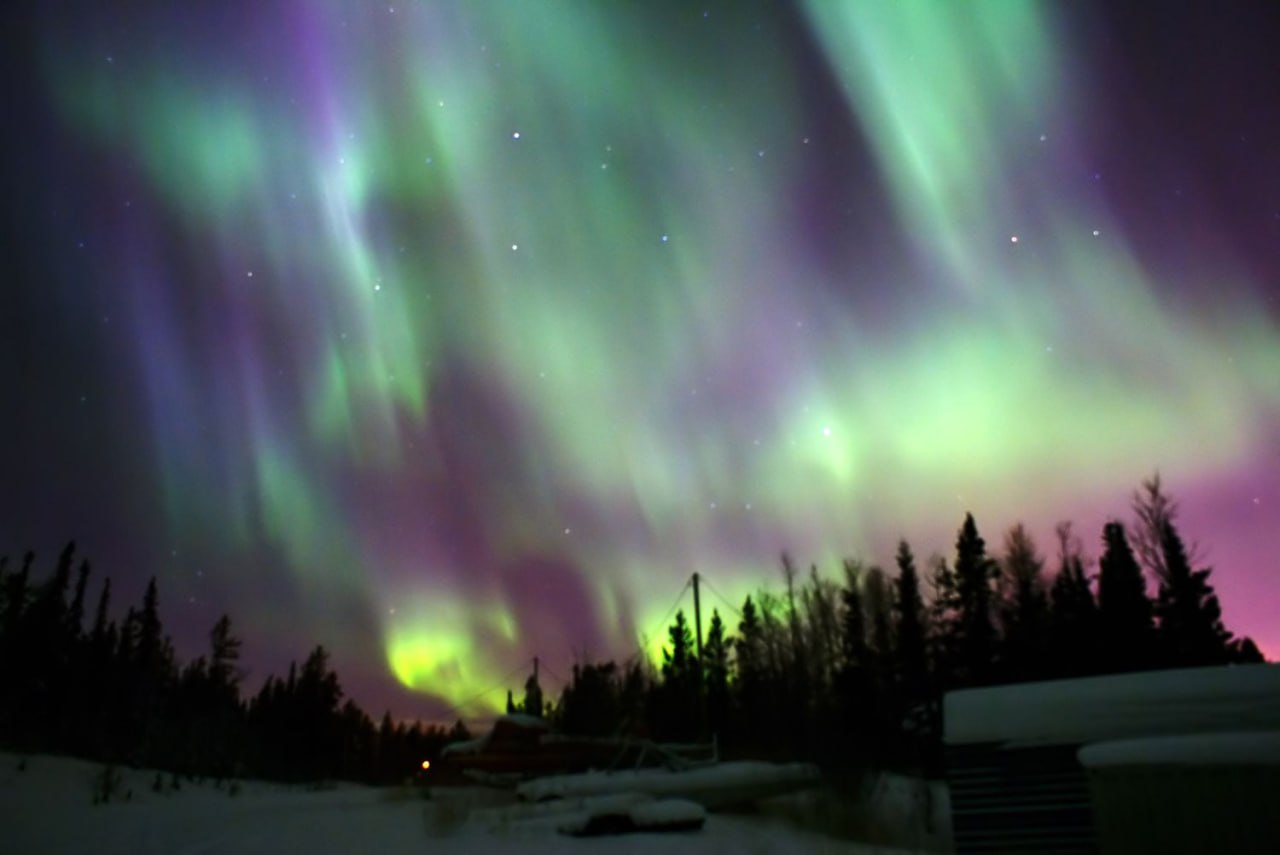
\includegraphics[width=0.8\textwidth]{images/aurora2.jpg}
    \caption{Дискретное полярное сияние (дуги и лучи)}
    \label{fig:aurora2}
\end{figure}